%=============================================================
\subsubsection{Perceptron.}

The theory behind artificial neural networks started with the model of \emph{Perceptron} introduced by \citet{mcculloch1943logical}. It is a simple model which transforms a vector of inputs $s$ to an output value $y$. 

\begin{figure}[h]
  \centering
  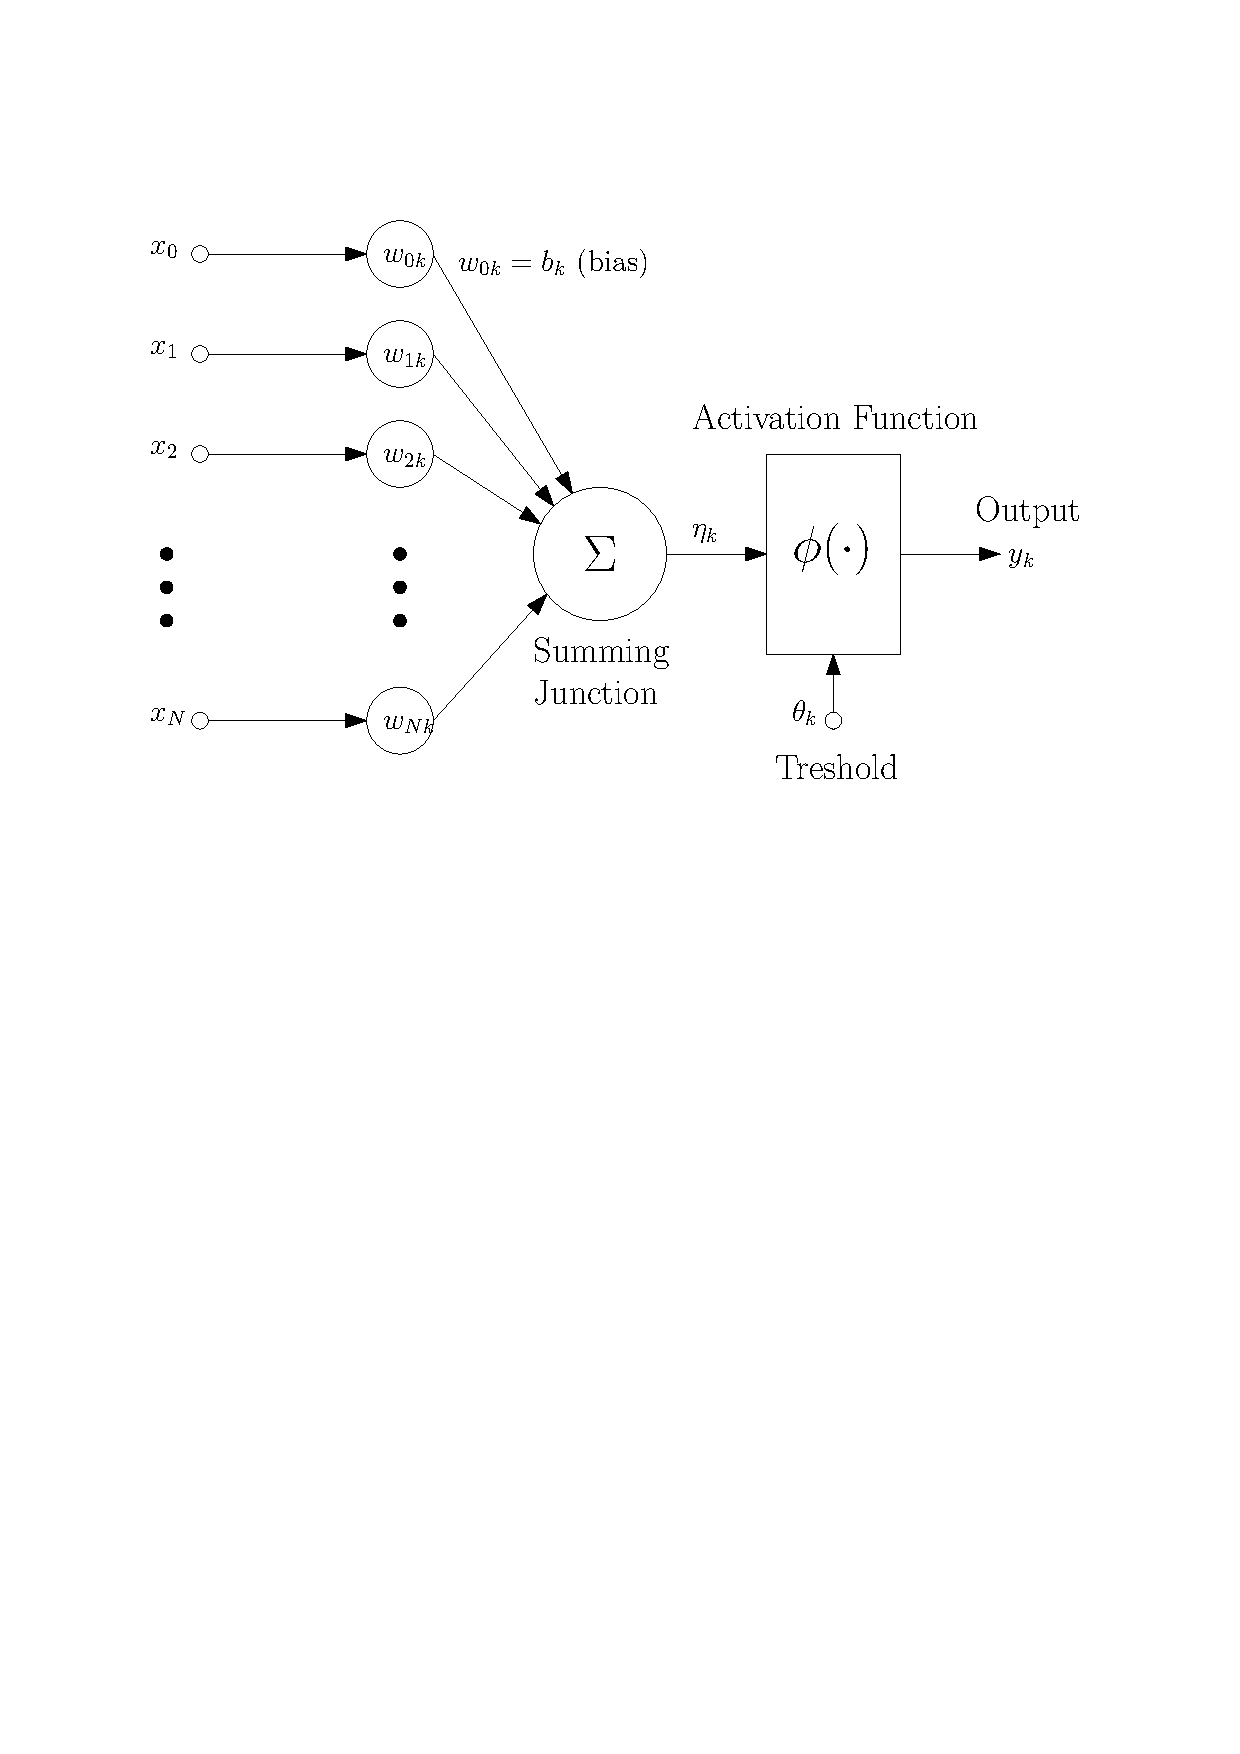
\includegraphics[width=0.7\textwidth]{img/perceptron.pdf}    
  \caption{Perceptron. Notation: $x$ is the \emph{input vector} where always $x_0=1$, $w_{0k}$ is the \emph{weight} vector, $\Sigma$ is the \emph{summing} junction, $eta_k$ is the \emph{net input}, $\phi$ is the \emph{activation function}, $\theta_k$ is the \emph{treshold}, $y_k$ is the \emph{output} and $b_k$ is the \emph{bias}.} 
  \label{fig:perceptron}
\end{figure}

The whole transformation of the input vector to the output activation could be written as follows: 
\begin{equation}
\label{eq:perceptron} 
y_k =
\left\{
	\begin{array}{ll}
		0 & \mbox{if } \phi(\sum_{i=0}^N x_iw_{ik}) < \theta_k \\
		1 & \mbox{otherwise}
	\end{array}
\right.
\end{equation} 

Equation~\ref{eq:perceptron} describes a simple \emph{binary treshold perceptron}. One could observe that the binary perceptron divides the vector space $\mathbb{R}^N$ by a $(n-1)$--dimensional hyperplane. This behaviour was studied by \citet{rosenblatt1958perceptron}. Now we see the importance of bias which is the absolute term in the equation of the hyperplane. 

\paragraph{Continuous perceptron.}
We put additional constraints for the activation function $\phi \mathbb{R} \mapsto (0,1)$: 
\begin{enumerate} 
\item It is differentiable and monotonously increasing,
\item and satisfying two asymptotic conditions $t(-\infty)=0$ and $t(\infty)=1$. 
\end{enumerate} 
Usually, the transfer function is realized by the logistic function: 

\begin{equation}
\frac{1}{1 + e^{-\eta}}. 
\end{equation} 

To allow the outputs to be from range $(0,1)$ we drop the treshold and simply output $\phi(\eta_k)$. 

\paragraph{Learning.} 
The goal of a perceptron is to \emph{learn} a given set $T = \{(X^j, t_j)\}$ mappings, where $X^j$ is the input vector $(x_{j0},x_{j1}, \ldots, x_jN)$ and $t_j$ is the corresponding target. Ideally, we want from the perceptron to be able generalize for novel inputs. The goal is formalized by minimizing an error function: 

\begin{equation}
\label{eq:perceptron-error} 
E = \sum_{k=1}^{N} \frac{1}{2}(y_k-t_k)^2.
\end{equation} 

A straightforward method to achieve this is simply updateing weights according to the partial derivates of the error function: 

\begin{equation}
\label{eq:perceptron-learning} 
\frac{\partial E}{\partial w_{ik}} = (y_k - t_k)\phi'(\eta_k)x_i = (y_k - t_k)y_k(1 - y_k)x_i.
\end{equation} 

From equation~\ref{eq:perceptron-learning} we can develop a following learning algorithm: 
\begin{figure}[h]
  \centering
\begin{lstlisting}
for e from 1 to EPOCHS: 
  foreach (X^j, t_j) in T: 
    calculate y_j
    for i from 0 to N: 
      update w_{ij}
\end{lstlisting}
  \caption{Perceptron learning. Developed from equations~\ref{eq:perceptron-error} and \ref{eq:perceptron-learning} we get an \emph{weight update} rule which is applied in loop for element in $T$. TODO sth better than lstlisting} 
  \label{fig:perceptron-learning}
\end{figure}

Usually, the \emph{update rule} is written as: 
\begin{equation} 
\Delta w_{ik} = \lambda (y_k - t_k)y_k(1 - y_k)x_i,
\end{equation} 
where $\lambda$ is the \emph{learning speed}. 

